\section{Animación de anatomía humana} 
\label{anatomy}

\todo{Esto esta bien, o asumimos que esto se sabe?}
\subsection{Introducción}
Antes de continuar, se va a introducir dos conceptos necesarios para la mejor compresión de las siguientes secciones. 
Es posible representar un modelo tridimensional en un computador de varias maneras. La más común es usar malla poligonal que representa la superficie del modelo que se quiere mostrar. Esta malla generalmente está compuesta de polígonos llamados facetas o caras que son la unidad básica de un modelo tridimensional. Las caras más comunes son los triángulos, siendo este el polígono más simple y rectángulos que se pueden descomponer en dos triángulos. Esta figura es la que más se usa debido a su adecuación de su complejidad matemáticas que ha hecho que las tarjetas gráficas se hayan diseñado con especial énfasis en el tratamiento de triángulos.
Por otra parte, se puede hacer uso de una representación volumétrica que  permite una representación visual completa de un objeto a través de las tres dimensiones físicas permitiendo visualizar tanto el exterior como el interior que la representación superficial no era capaz. Sin embargo, esto produce una gran complejidad al intentarlas representar mediante imagen generada por computador.
En la figura \ref{fig:HVP} se puede apreciar las dos representaciones del mismo modelo anatómico.

\begin{figure}[h]
   \centering
    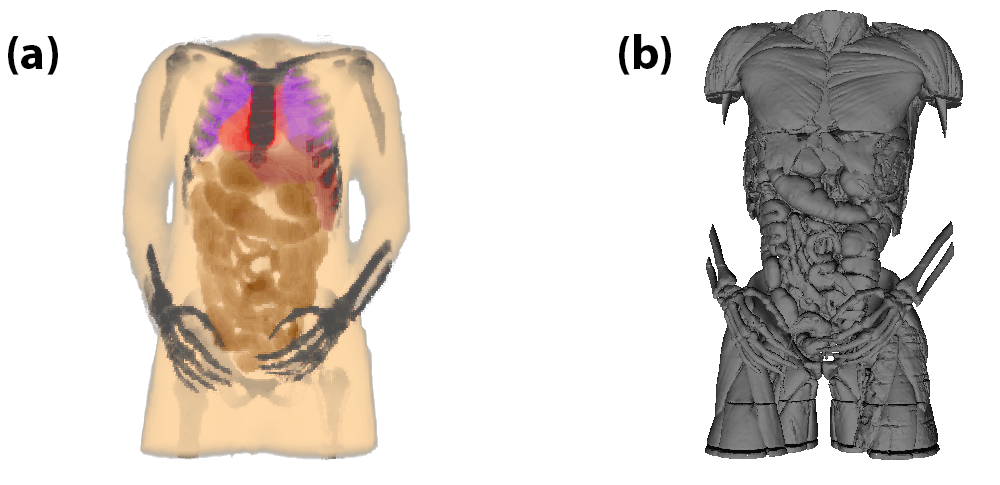
\includegraphics[width=0.5\textwidth]{IMG/volvsb-rep.png}
    \caption{La figura (a) muestra la representación volumétrica del \emph{Visible Human Project}\cite{ackerman1998visible}. La figura (b) muestra la malla poligonal del mismo modelo. }
   \label{fig:HVP}
\end{figure}
\todo{hace falta explciar la malla de tetraedros?}
Una de las necesidades básicas de un simulador para ser realista es que la información anatómica de los pacientes virtuales con las que trabajará el usuario sean realistas. Para ello se necesita seleccionar un modelo anatómico realista en alguna representación anteriormente comentada. Además, también se busca que la experiencia sea lo más cercana a la realidad posible y a la vez que contemple una gran variedad de casos. En  \cite{preim2018survey} se explica la necesidad de que los estudiantes tengan un conocimiento profundo de la anatomía humana, estructuras, su posición relativa, variabilidad, etc... En este artículo se presenta un resumen de técnicas de visualización e interacción desarrolladas para este fin.

Respecto a los modelos humanos virtuales, existen varios modelos comerciales como puede ser \emph{ZygoteBody}$^{TM}$ ~\cite{kelc2012zygote}, \emph{Anatomium} ~\cite{Anatomium},   \emph{BioDigital Human} \cite{qualter2012biodigital}o modelos como \emph{Visible body}\cite{visible2012visible} que solo está centrado en músculos y deformaciones predefinidas. Estos modelos han sido  diseñados por artistas representan cánones no realistas que no reflejan fielmente la anatomía de los pacientes a las que podría enfrentarse un médico. Para ello, en la actualidad se sigue investigando para llevar datos de pacientes reales a modelos virtuales y de esta forma usar datos capturados usando técnicas de imagen médica (como CT, MRI o US). Existen incluso representaciones volumétricas casi completas como son el \emph{Visible Human Project}\cite{ackerman1998visible}  y un modelo basado en este llamado \emph{Segmented Inner Organs}\cite{VoxelMan}. Sobre estos datos capturados, muchos investigadores han propuesto métodos para llevar esto acabo y se pueden consultar \cite{ferrante2017slice}.

Tanto los modelos comerciales como los modelos obtenidos a través de imagen médica, presentan el mismo problema: los modelos son presentados en una misma postura, que suele coincidir con la postura de adquisición. Esto hace que los datos de pacientes sean estáticos y limitados que no representan la mayoría de los casos. Es en algunos procedimientos médicos como puede ser la artroscopia de rodilla, las imágenes capturadas no presentan la misma postura que será necesaria para el procedimiento adecuado, ya que se necesita la rodilla flexionada frente a la pierna extendida donde fue capturada la imagen. 

Es importante remarcar que la mayoría de las técnicas que se presentan en \cite{ferrante2017slice} no son capaces de capturar adecuadamente todos y cada uno de los tejidos del paciente. En ocasiones solo se centran en tejidos concretos como puede ser la piel y músculos en general. Además, las técnicas actuales de imagen médica tampoco son capaces de recuperar las propiedades mecánicas de todos los tejidos siendo esto un gran inconveniente al intentar simular fielmente estos datos.

Por tanto, estos simuladores necesitaran un método que pueda tratar datos de personas con todos los tejidos internos, de esta manera se podrá reproducir todo tipo de posturas, posiciones y, en resumen, generar variabilidad para que los usuarios puedan entrenar un gran número de posibilidades en los simuladores médicos.




\subsection{Animación de personajes} 
\label{art:animation}

En esta sección se presentan una visión general de los diferentes algoritmos existentes para animar modelos tridimensionales. La animación consiste en deformar la representación B-rep o volumétrica por medio de modelos matemáticos. Estos modelos matemáticos pueden ser clasificados de dos tipos, aquellos que tienen en cuenta las propiedades físicas del modelo y aquellos que solo utilizan operaciones geométricas para animar el modelo. Actualmente, es habitual que los algoritmos geométricos esta orientados a ser interactivos sacrificando deformaciones físicamente correctas y los algoritmos físicos están centrados en una deformación más realista.  Aun así, existen algoritmos que combinan ambos enfoques para conseguir deformaciones más realistas con tasas interactivas, o reducir el tiempo de procesado mientras se mantiene el comportamiento físico. 


\subsection{Animación esqueletal}
\label{art:virtualskel}

La animación esqueletal es un método geométrico que anima un modelo representado por su malla superficial, normalmente llamada piel, y un esqueleto virtual formado por huesos ordenados jerárquicamente. Asociando los vértices a los distintos huesos, esta técnica permite transferir el movimiento del esqueleto a su piel. Esta técnica fue introducida por Nadia Magnenat en 1988 \cite{thalmann88} y sigue siendo la técnica más utilizada debido a su sencillez y su fácil adaptación al cauce gráfico. A pesar de la existencia de métodos más realistas, esta técnica se usa prácticamente en todos los sistemas de animación ya que simplifica el trabajo de los artistas o es el paso previo a algoritmos más complejos. Por ejemplo, se puede animar mediante captura de movimientos y cinemática inversa entre otros.

the virtual skeleton is a mathematical
abstraction used to define the rotation point of the different VPH model joints.
These rotation points are called virtual joints and they are hierarchically
structured.
Magnenat-Thalmann et al in their seminal paper [1] describe how virtual
skeletons can be applied to animate 3D meshes. Figure 3 shows an example
of a virtual skeleton superimpose to the virtual patient bones and skin. The
grey spheres represent the virtual joints, while the grey prisms represent the
hierarchical relationship among the virtual joints.

\begin{figure}[h]
   \centering
    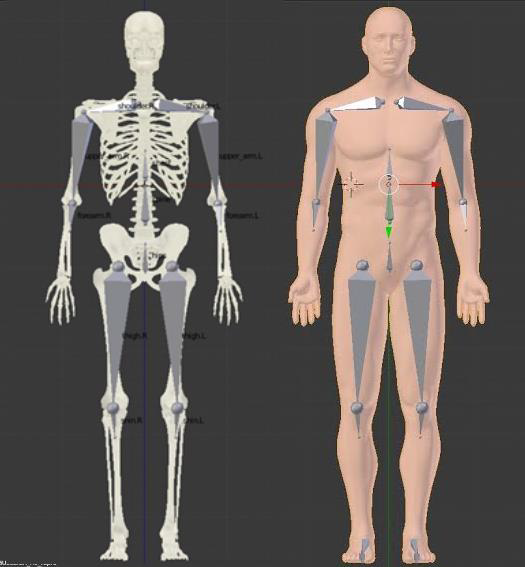
\includegraphics[width=0.5\textwidth]{IMG/virtualskeleton.png}
    \caption{ }
   \label{fig:zygoteproblems}
\end{figure}

Con el paso del tiempo, se han definido los siguientes conceptos en los que se puede dividir la animación esqueletal:

\begin{itemize}
    \item \emph{Rigging}\footnote{Término utilizado en la industria para la creación o adaptación del esqueleto virtual \label{footnote1}}: En esta etapa se crea el esqueleto virtual específicamente para el modelo que queramos animar
    \item Pesado: Una vez creados los huesos virtuales, se asigna el peso de influencia de cada hueso para cada vértice de la piel del modelo.
    \item \emph{Skinning}\textsuperscript{\ref{footnote1}}: Se define las operaciones matemáticas que van a transferir el movimiento de los huesos 
    \item Animación: Se mueven los huesos y esto produce una deformación en la piel.
\end{itemize}

A continuación se mostrará la revisión de la literatura existente para cada etapa.
\subsubsection{Rigging}
\label{art:rigging}

El proceso de \emph{rigging} consiste en crear un esqueleto virtual lo más cercano a el esqueleto original que tuviera el modelo tridimensional que se esta animando. Este trabajo normalmente es realizado por un artista ayudado de un programa CAD (siglas en ingles de diseño asistido por computador) como puede ser \emph{Blender} \cite{a}, herramientas de \emph{Autodesk} como pueden ser \emph{Maya} o \emph{3DS MAX} \cite{a}. También existen algunos trabajos que tratan de automatizar el proceso de creación de esqueletos virtuales siguiendo dos enfoques: adaptando esqueleto predefinido \cite{a} o infiriendo el esqueleto en base a la malla superficial \cite{a}.
Existen limitaciones para aquellos esqueletos virtuales que solo se definen por rotaciones, ya que los movimientos de modelos orgánicos son mucho más complejos. Algunos trabajos intentan definir articulaciones basado en modelos anatómicos \cite{joints} con \emph{splines}\footnote{ es una curva diferenciable definida en porciones mediante polinomios} mejorando el movimiento del hueso pero dificultando la creación del esqueleto virtual y el proceso de manipulación.
Currently, there exist several techniques to adapt a generic virtual skeleton to a 3D character~\cite{huang2013robust,feng2014fast,pan2017automatic}.


\subsubsection{Pesado}
\label{art:pesado}

Este proceso  determina cual es la influencia de cada hueso virtual en cada vértice de la malla superficial. El cálculo de esta influencia se denomina pesado al determinar que un vértice lleva asociado una serie de pesos $w_{i,j}$ que relacionan un vértice $i$ con el hueso $j$.
Para asegurar una deformación correcta se presuponen las siguientes condiciones que tienen que cumplir el pesado:
\begin{eqnarray}
%\begin{equation}
\label{cond1}
w_{i,j}\geq 0 \;\;\;\;\;\;\;\; \forall i \in V \wedge \forall j \in B   \\
%\end{equation}
%\begin{equation}
\label{cond2}
\sum_{j \in B} w_{i,j} = 1\ \;\;\;\;\;\;\;\;\;\;\;\;\;\;\;\;
\forall i \in V
%\end{equation}
\end{eqnarray}
Donde V es el conjunto de vértices de la malla poligonal y B son el conjunto de huesos en el esqueleto virtual. No puede existir un hueso que influya negativamente a un vértice, por ello se tiene que cumplir la condición \ref{cond1}. Además, para garantizar que no se genere movimientos extra, es necesario cumplir la condición \ref{cond2}.
Por último, resulta intuitivo pensar que las transiciones entre huesos virtuales deberían ser progresivas, el gradiente de los pesos debe ser suave, para evitar efectos extraños y discontinuidades en la malla.

Originalmente, al igual que la etapa anterior, un artista era el encargado de realizar la tarea manualmente, donde se utilizaban herramientas \emph{CAD} para \emph{pintar} la influencia de un hueso en la malla superficial. Actualmente en la literatura se pueden encontrar métodos semi-automáticos\cite{a} y también totalmente automáticos \cite{}. 
Algunos de estos trabajos no tienen en cuenta la conectividad de la malla y puede ser que haya vértices topológicamente lejanos con pesos similares. Se han propuesto soluciones como \cite{Baran:2007} utilizando ecuaciones diferenciales que ayudan a calcular transiciones más suaves en la malla. Esta solución es más compleja (resolución de sistemas de ecuaciones, cálculo de vecindad, etc) pero ofrece transiciones más realistas y menor intervención manual.

explain the properties the weights $w_{i,j}$ must meet: (i) the vertex weights must be independent of the mesh topology or resolution; (ii) the weights must vary smoothly along the volume. In order to ensure these two properties, they proposed to use Laplace diffusion equation.

\emph{Baran and Popovi\'{c}}~\cite{Baran:2007} propose an algorithm to automate both rigging and weighting stages. In their work, they adapt a previous generated virtual skeleton to a 3D model. Then, the influences of the virtual bones over the vertex of the surface mesh are computed using Laplace diffusion equation. This technique is constrained to B-Rep models and the surface mesh must completely enclose the virtual skeleton. 
The weighting phase of our animation pipeline extends this technique to deal with the internal anatomy of the model and to take into account the models’ bone tissue for building the virtual skeleton.
\emph{Baran and Popovi\'{c}}~\cite{Baran:2007} propose an algorithm to automate both rigging and weighting stages. In their work, they adapt a previous generated virtual skeleton to a 3D model. Then, the influences of the virtual bones over the vertex of the surface mesh are computed using Laplace diffusion equation. This technique is constrained to B-Rep models and the surface mesh must completely enclose the virtual skeleton. 
The weighting phase of our animation pipeline extends this technique to deal with the internal anatomy of the model and to take into account the models’ bone tissue for building the virtual skeleton. 
\emph{Jacobson et al.}~\cite{Jac2011} improve the weighting phase to deal with point handles, virtual bones and cages. They minimize the Laplacian energy subject to the handles' constraints (among other constraints) to achieve high-order smoothness (see equation \ref{eqn:1}):
\begin{equation}
\label{eqn:1}
\mathrm{arg\,min}_{W_j, j=1..m}\sum_{j}^m\frac{1}{2}\int_\Omega \left \|  \nabla W_j\right \|^2 dV,
\end{equation}
where $W_j$ are the weights of the handle $j$ and $m$ is the number of handles. 

\subsubsection{Skinning}
\label{art:skinning}

\subsection{Animación basada en físicas}